% !TEX encoding = UTF-8 Unicode
\documentclass[a4paper]{article}

\usepackage[utf8]{inputenc}
\usepackage[francais]{babel}
\usepackage[nonewpage]{imakeidx}
\usepackage{hyperref}
\usepackage{enumitem}
\usepackage{graphicx}
\usepackage{array}
\usepackage{float}

% Glossaire:
\usepackage[acronym,toc,nopostdot, nonumberlist]{glossaries}
% !TEX encoding = UTF-8 Unicode
% Glossaire
\newglossaryentry{joueur}
{
    name=joueur,
    description={Personnage fictif du jeux pouvant faire partie d'une équipe et jouant au quiditch.}
}
\newglossaryentry{equipe}
{
    name=équipe,
    description={Elle est composée de 7 \glspl{joueur} (un gardien, un attrapeur, deux batteurs et trois poursuive).}
}
\newglossaryentry{manager}
{
    name=manager,
    description={\Gls{utilisateur} du programme, il possède un \gls{club} et dois faire en sorte que celui-ci gagne de l'argent.}
}
\newglossaryentry{club}
{
    name=club,
    description={Infrastructure contenant une \gls{equipe} et des installations (stade, infirmerie,\ldots).}
}

\newglossaryentry{utilisateur}
{
    name=utilisateur,
    description={Personnage réel. C'est la personne qui joue au Quiditch manager.\\
    Elle est appelée en jeu \gls{manager}}
}

\newglossaryentry{enchere}
{
    name=enchère,
    description={Système permettant l'achat de \glspl{joueur}}
}
\newglossaryentry{serveur}
{
    name=serveur,
    description={Programme étant toujours en marche et connecté à internet et qui réceptionne les connections des \glspl{client}. Il a les données de tous les \glspl{utilisateur}.}
}
\newglossaryentry{client}
{
    name=client,
    description={Programme que l'\gls{utilisateur} lance pour se connecter au \gls{serveur}. Il permet à l'\gls{utilisateur} de jouer et peut être soit en ligne de commande, soit en mode graphique.}
}
\newglossaryentry{participant}
{
    name=participant,
    description={Nom donné à l'\gls{utilisateur} lors d'un tournoi.}
}


% Acronymes

\makeglossaries
\setglossarysection{subsection}
\deftranslation{Glossary}{Glossaire}
\renewcommand*{\glossaryname}{Glossaire}
\DeclareRobustCommand{\gloss}[1]{\it{#1}\index{\glslabel}}
\renewcommand{\glsdisplay}[4]{\gloss{#1#4}}
\renewcommand{\glsdisplayfirst}[4]{\gloss{#1#4}}


\makeindex
\indexsetup{level=\section}
\setcounter{secnumdepth}{4}

\title{Quiddich live : \\Software requirements document}
\author{Bruno Rocha Pereira \and Jérome Vial \and Cédric Strebelle \and
Romain Fontaine \and Tsotne Shonia \and Nikita Marchant}
\date{\today}

% Début du document
\begin{document}

\maketitle

\section{Introduction}
\subsection{But du projet}
Le but du projet d'année en BA2 en sciences informatiques est le développement d'une application de jeu multijoueur en ligne.
Il consiste en l'implémentation d'un jeu de Quidditch, sport tiré de la saga Harry Potter de J.K.Rowling.

 
Le Quidditch est un sport pratiqué par deux \glspl{equipe} de 7 \glspl{joueur} évoluant à l'aide de leur balais sur un terrain de forme ovale. Le but de ces 2 \glspl{equipe} est de marquer le plus de points possible en marquant à l'aide du souaffle dans un des 3 buts adverses et d'attraper le vif d'or\footnote{Pour plus d'informations, se référer au livre J. K. Rowling : "Le Quidditch à travers les âges", Gallimard, 2001.}, qui qui signe la fin du match. 


Notre application sera un jeu de gestion et stratégie en ligne, se jouant individuellement pendant la gestion et au tour par tour à 2 joueurs lors des matchs. L'\gls{utilisateur} est le \gls{manager} d'un \gls{club} de Quidditch et son but est de faire progresser son \gls{club} vers le succès. Pour ce faire, il devra gérer tous les aspects du \gls{club}, tant au niveau sportif que financier. Il aura à sa disposition différentes installation pour entraîner ses \glspl{joueur} ou gagner de l'argent. Il pourra améliorer les différentes installation de son \gls{club} à l'aide d'argent.

Cet argent sera récolté lors des matchs et dans les magasins du \glspl{club}. La saison de Quidditch se déroule sous la forme d'un championnat, durant lequel tous les \glspl{utilisateur} inscrits s'affrontent entre eux au cours de matches. Les matches seront planifiés dans un calendrier qu'il faudra respecter sous peine de sanction. Un match se joue au tour part tour, mais les deux \glspl{utilisateur} jouent simultanément, le \gls{serveur} résolvant les conflits à la fin de chaque tour. Il y a donc une notion importante d'anticipation dans la maîtrise de ce jeu.

En ce qui concerne la gestion du \gls{club}, l'\gls{utilisateur} aura la possibilité de recruter de nouveaux \glspl{joueur} de Quidditch pour renforcer son \gls{equipe}, il pourra aussi développer différentes infrastructures et services comme son stade, son infirmerie, son terrain d'entraînement, son fanshop etc.

% glossaire
\printglossary[numberedsection]
\subsection{Historique}
\begin{description}
\item[0.1] (05/12/13) : Création du document
\item[0.2] (10/12/13) : Premier jet de chaque partie
\item[0.3] (11/12/13) : Création des diagrammes UML
\item[0.4] (12/12/13) : Ajout du glossaire
\item[0.5] (19/12/13) : Corrections et ajout des diagrammes au document
\item[1.0] (20/12/13) : Délivrable pour la phase 1
\end{description}

\section{Besoins d'utilisation}
\subsection{Exigences fonctionnelles}

\subsubsection{Identification}

\paragraph{Inscription (fig \ref{diag-use-inscription})}

\begin{figure}[H]
   \begin{center}
   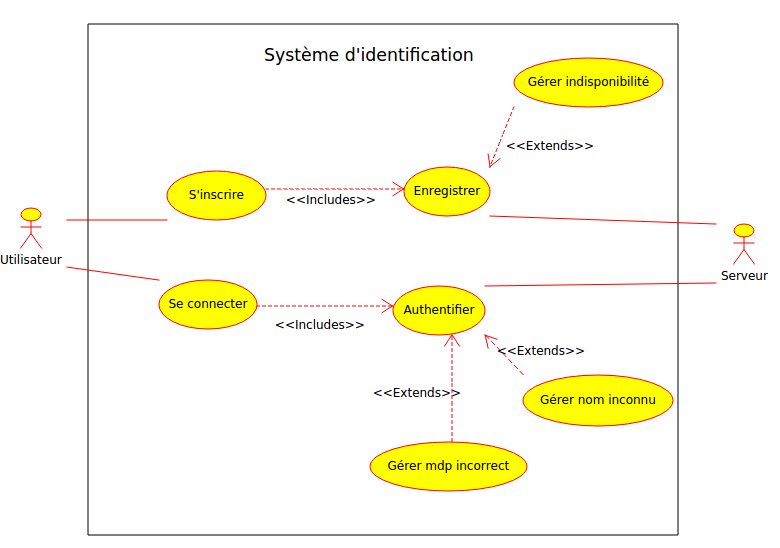
\includegraphics[height=250pt]{uml/id.png}
   \caption{\label{diag-use-inscription} Système d'identification}
   \end{center}
\end{figure}

\begin{description}
\item[Cas général  :] L'\gls{utilisateur} doit pouvoir s'inscrire (s'enregistrer) sur le \gls{serveur} avec un nom d'\gls{utilisateur} unique et un mot de passe.
\item[Pré Condition  :] Néant.
\item[Post Condition :] L'\gls{utilisateur} aura fait une demande d'inscription.
\item[Cas Exceptionnel :] L'inscription échouera et l'\gls{utilisateur} sera invité à recommencer si le nom de compte est déjà enregistré sur le \gls{serveur}.
\end{description}

\paragraph{Connection (fig \ref{diag-use-inscription})}
\begin{description}
\item[Cas général :] L'\gls{utilisateur} doit pouvoir se connecter en s'authentifiant auprès du \gls{serveur} avec son nom d'\gls{utilisateur} et son mot de passe.
\item[Pré Condition  :] Néant.
\item[Post Condition :] L'\gls{utilisateur} aura fait une demande de connexion.
\item[Cas Exceptionnel :] L'authentification échouera et l'\gls{utilisateur} sera invité à recommencer si le mot de passe ne correspond pas au nom d'\gls{utilisateur}, ou cet \gls{utilisateur} n'existe sur le \gls{serveur}.
\end{description}

\subsubsection{Gérer le \gls{club} (en phase de management)}

\begin{figure}[H]
   \begin{center}
   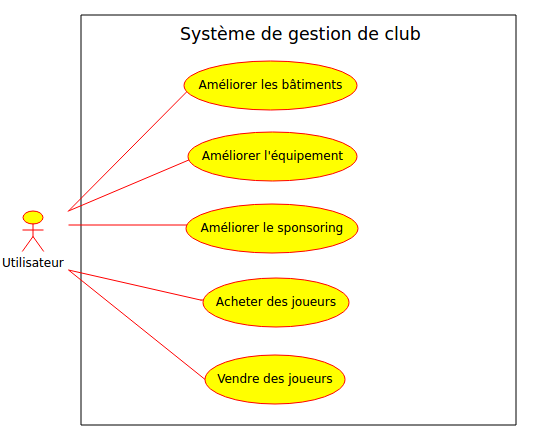
\includegraphics[height=250pt]{uml/mngClub.png}
   \caption{\label{diag-use-management} Gestion d'un \gls{club} pendant la phase de management}
   \end{center}
\end{figure}

\paragraph{Améliorer les bâtiments}
\begin{description}
\item[Cas général :] L'\gls{utilisateur} doit pouvoir améliorer ses divers bâtiments sur plusieurs niveaux. 
\item[Pré Condition  :] L'\gls{utilisateur} doit être connecté.
\item[Post Condition :] Chaque bâtiment a sa ou ses spécificités, parmi ces trois-ci :
	\begin{itemize}
	\item Améliorer la rentrée d'argent.
	\item  Améliorer l'entraînement (les caractéristiques) des \glspl{joueur}.
	\item  Apporter des soins plus efficaces aux \glspl{joueur}.
	\end{itemize}
\item[Cas Exceptionnel :] Une dépense n'est pas acceptée si le \gls{club} de l'\gls{utilisateur} ne dispose pas de suffisamment d'argent pour l'effectuer.
\end{description}

\paragraph{Améliorer l'équipement}
\begin{description}
    \item[Cas général :] L'\gls{utilisateur} doit pouvoir améliorer l'équipement de ses \glspl{joueur} (bâtons, ...).
    \item[Pré Condition  :] L'\gls{utilisateur} doit être connecté.
    \item[Post Condition :] L'équipement (et donc les statistiques) des \glspl{joueur} seront modifiées.
    \item[Cas Exceptionnel :] Une dépense n'est pas acceptée si le \gls{club} de l'\gls{utilisateur} ne dispose pas de suffisamment d'argent pour l'effectuer.
\end{description}

\paragraph{Améliorer le sponsoring}
\begin{description}
\item[Cas général :] L'\gls{utilisateur} doit pouvoir améliorer son sponsoring et les détails relatifs pour sa rentrée d'argent.
\item[Pré Condition  :] L'\gls{utilisateur} doit être connecté.
\item[Post Condition :] Le sponsoring, et donc une source de rentrée d'argent sera modifiée.
\item[Cas Exceptionnel :] Une dépense n'est pas acceptée si le \gls{club} de l'\gls{utilisateur} ne dispose pas de suffisamment d'argent pour l'effectuer.
\end{description}

\paragraph{Acheter des \glspl{joueur}}
\begin{description}
    \item[Cas général :] L'\gls{utilisateur} doit pouvoir acheter des \glspl{joueur}.
    \item[Pré Condition  :] L'\gls{utilisateur} doit être connecté.
    \item[Post Condition :] L'\gls{equipe} de l'\gls{utilisateur} sera modifiée.
    \item[Cas Exceptionnel :] Une dépense n'est pas acceptée si le \gls{club} de l'\gls{utilisateur} ne dispose pas de suffisamment d'argent pour l'effectuer.
\end{description}

\paragraph{Vendre des \glspl{joueur}}
\begin{description}
    \item[Cas général :] L'\gls{utilisateur} doit pouvoir vendre l'un (ou plusieurs) de ses \glspl{joueur}.
    \item[Pré Condition  :] L'\gls{utilisateur} doit être connecté.
    \item[Post Condition :] L'\gls{utilisateur} obtiendra de l'argent. Son \gls{equipe} sera modifiée.
\end{description}

\subsubsection{Jouer en tournoi}
\begin{figure}[H]
   \begin{center}
   \caption{\label{diag-use-championship} Diagramme d'utilisation : gestion des tournois}
   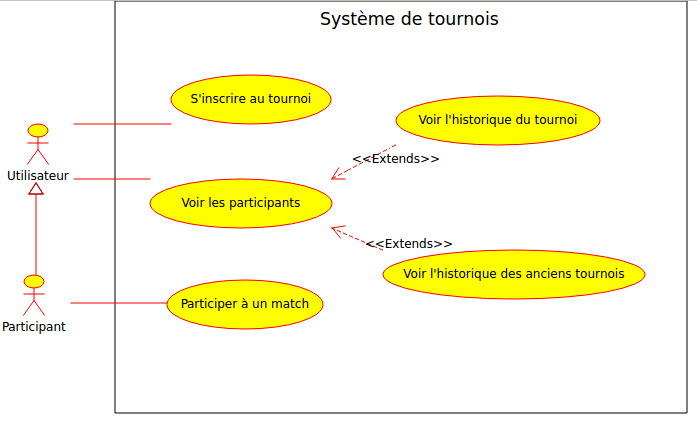
\includegraphics[height=250pt]{uml/usrTournoi.png}
   \end{center}
\end{figure}
\paragraph{S'inscrire en tournoi}
\begin{description}
\item[Cas général :] L'\gls{utilisateur} doit pouvoir s'inscrire à un tournoi dont la date limite des inscriptions n'est pas encore passée.
Ce qui lui permettra d'être sélectionné pour des matches et d'y affronter les autres \glspl{participant} inscrits à ce tournoi.
\item[Pré Condition  :] L'\gls{utilisateur} doit être connecté.
\item[Post Condition :] L'\gls{utilisateur} sera inscrit pour le tournoi.
\item[Cas Exceptionnel :] Un \gls{utilisateur} ne peut pas se réinscrire dans un tournoi auquel il est déjà inscrit.
\end{description} 

\paragraph{Participer à un match du tournoi}
\begin{description}
\item[Cas général :] L'\gls{utilisateur} doit pouvoir participer à un match en ligne du tournoi où il affrontera le \gls{participant} adverse.
\item[Pré Condition  :] L'\gls{utilisateur} doit être connecté et sélectionné comme étant l'un des deux \gls{participant} du match.
\item[Post Condition :] L'\gls{utilisateur} sera en match contre le \gls{participant} adverse.
\item[Cas Exceptionnel :] L'\gls{utilisateur} sera considéré comme perdant automatiquement s'il a déclaré forfait.
\end{description}

\subsubsection{Voir les informations relatives à un tournoi}
\paragraph{Voir la liste des \glspl{participant} d'un tournoi}
\begin{description}
\item[Cas général :] L'\gls{utilisateur} doit pouvoir voir la liste des \glspl{participant} d'un tournoi lancé ou terminé.
\item[Pré Condition  :] L'\gls{utilisateur} doit être connecté.
\item[Post Condition :] Néant.
\end{description}
\paragraph{Voir l'historique d'un tournoi}
\begin{description}
    \item[Cas général :] L'\gls{utilisateur} doit pouvoir voir l'historique d'un tournoi lancé ou terminé, c'est à dire l'arbre du tournois de ce dernier avec des détails concernant les \glspl{equipe}.
    \item[Pré Condition  :] L'\gls{utilisateur} doit être connecté et ne doit pas être en plein match.
    \item[Post Condition :] Néant.
\end{description}

\subsubsection{Jouer à un match}
\paragraph{Jouer un tour}
\begin{description}
    \item[Cas général :] L'\gls{utilisateur} doit pouvoir jouer un tour lors d'un match, c'est à dire déplacer ses \glspl{joueur} et/ou effectuer des actions.
    \item[Pré Condition  :] L'\gls{utilisateur} doit être entrain de jouer à un match.
    \item[Post Condition :] L'\gls{utilisateur} aura joué son mouvement.
    \item[Cas Exceptionnel :] La perte de connexion avec un \gls{utilisateur} maintenue, durant un certain timeout, entraînera son remplacement pour ce match par une IA fournie par le système. Le match continuera sans changement.
\end{description}
\paragraph{Déclarer forfait}
\begin{description}
\item[Cas général :] L'\gls{utilisateur} peut déclarer forfait durant un match (il sera considéré comme perdant).
\item[Pré Condition  :] L'\gls{utilisateur} doit être entrain de jouer à un match.
\item[Post Condition :] L'\gls{utilisateur} sera déclaré comme perdant.
\end{description}

% fin de "Exigences fonctionnelles"
%%%%%%%%%%%%%%%%%%%%%%%%%%%%%%%%%%%

\subsection{Exigences non fonctionnelles}
\begin{itemize}
\item La machine hébergeant le \gls{client} ainsi que le \gls{serveur} doivent être en mesure de communiquer en permanence via un réseau capable de transporter des paquets \textbf{TCP/IP}
\item Le réseau décrit ci-dessus doit pourvoir une latence raisonnablement faible (c'est à dire de plus ou moins 200ms pour un aller retour)
\item Les machines exécutant le \gls{client} doivent être équipées d'un écran, d'un clavier et d'une souris et être capables d'afficher des images en mode graphique ainsi qu'au minimum 80 caractères de large en mode console. Elles devront aussi avoir au minimum disposer de 512Mb de mémoire vive ainsi que 500Mb d'espace disque.
\end{itemize}

% fin de "Exigences non fonctionnelles"
%%%%%%%%%%%%%%%%%%%%%%%%%%%%%%%%%%%%%%%

\subsection{Exigences de domaine}
\begin{itemize}
    \item Le jeu doit être multijoueur, les différents \glspl{utilisateur} connectés sur un même \gls{serveur} doivent pourvoir interagir entre eux.
    \item Le monde doit être persistent : il doit continuer d'évoluer, même en l'absence d'un ou plusieurs \glspl{utilisateur}.
    \item Une \gls{equipe} de Quiddich doit comporter 7 \glspl{joueur} au maximum, sans compter les remplaçants.
    \item Un \gls{joueur} blessé/mort ne peut être remplacé en plein match.
    \item Un match nécessite trois balles : Un souaffle, deux cognards et un vif d'or. Le terrain doit comporter deux buts, fait chacun de trois anneaux, et placé aux deux extrémités.
    \item Pour participer à un match, chaque \gls{joueur} doit avoir au moins un balai.
    \item Le match ne prend fin que si le vif d'or est attrapé ou que l'une des deux \glspl{equipe} abandonne.
    
\end{itemize}

% fin de "Exigences de domaine"
%%%%%%%%%%%%%%%%%%%%%%%%%%%%%%%%%%%%%%%

\section{Besoin du système}
\subsection{Exigences fonctionnelles}

\subsubsection{Identification}
\paragraph{Enregistrer une inscription}
\begin{description}
\item[Cas général :] Le système doit être capable d'enregistrer un nom de compte unique associé à un mot de passe dans un fichier, ainsi que de vérifier que le nom de compte fourni est unique.
\item[Pré Condition  :] Un \gls{utilisateur} effectuant une demande d'inscription.
\item[Post Condition :] Le nom de compte sera enregistré sur le \gls{serveur}. L'\gls{utilisateur} sera donc inscrit.
\item[Cas Exceptionnel :] L'enregistrement échouera si le nom de compte est déjà enregistré sur le fichier.
\end{description}

\paragraph{Authentifier}
\begin{description}
\item[Cas général :] Le système doit être capable d'authentifier un \gls{utilisateur} demandant de se connecter en vérifiant que le nom de compte fourni lors de la connexion est présente dans le fichier du \gls{serveur} et est bien associé au mot de passe fourni.
\item[Pré Condition  :] Un \gls{utilisateur} effectuant une demande de connexion.
\item[Post Condition :] L'\gls{utilisateur} sera connecté.
\item[Cas Exceptionnel :] L'authentification échouera si le nom de compte fourni n'est pas enregistré sur le \gls{serveur}, ou s'il est associé à un autre mot de passe que le mot de passe fourni.
\end{description}

\subsubsection{Interface}
\paragraph{Fournir une interface}
\begin{description}
\item[Cas général :] Le système doit fournir à l'\gls{utilisateur} une interface jeu simple, complète et interactive, graphique et en console pour les deux phases de jeu.
\item[Pré Condition  :] Néant.
\item[Post Condition :] Néant.
\end{description}

\paragraph{Représenter phase management}
\begin{description}
\item[Cas général :] Le système doit fournir à l'\gls{utilisateur} une représentation du \gls{club} (phase management), comprenant une vue d'ensemble sur son argent, ses rentrées, ses \glspl{joueur}, ses infrastructures et les améliorations possibles.
\item[Pré Condition  :] Néant.
\item[Post Condition :] Néant.
\end{description}

\paragraph{Représenter phase match}
\begin{description}
\item[Cas général :] Le système doit fournir à l'\gls{utilisateur} une représentation du terrain ovale (phase match), sous forme de cases hexagonales.
\item[Pré Condition  :] Néant.
\item[Post Condition :] Néant.
\end{description}

\subsubsection{Gestion de tournois}
\begin{figure}[h]
   \caption{\label{1} Gestion de tournois.}
   \begin{center}
   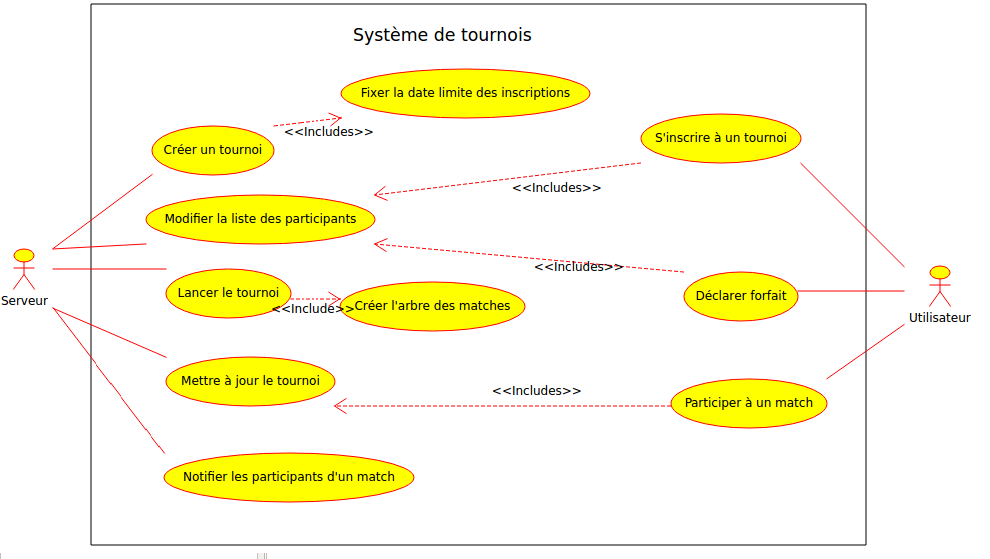
\includegraphics[height=250pt]{uml/servTournoi.png}
   \end{center}
\end{figure}
\paragraph{Créer un tournoi}
\begin{description}
\item[Cas général :] Le système doit créer les tournois avec un certain intervalle de temps, où les \glspl{utilisateur} pourront s'inscrire et devront s'affronter durant des matches organisés dans les stades des \glspl{club}.
\item[Pré Condition  :] Néant.
\item[Post Condition :] Un tournoi sera crée et mit en phase d'attente.
Durant sa création, il fixera une date limite pour les inscriptions.
\end{description}

\paragraph{Modifier la liste des \glspl{participant}}
\begin{description}
\item[Cas général :] Le système doit gérer une liste des \glspl{participant}, indiquant quel \gls{utilisateur} participe ainsi que son état (éliminé, en course). Le système doit être capable de le modifier la liste durant les inscriptions et après que le tournoi soit lancé.
\item[Pré Condition  :] Un tournoi en attente ou lancé.
\item[Post Condition :] La liste des \glspl{participant} d'un tournoi sera modifiée.
\end{description}

\paragraph{Lancer le tournoi}
\begin{description}
\item[Cas général :] Lorsque la date limite d'une phase d'inscription tournoi en attente est atteinte, le système doit générer l'arbre du tournois et lancer le dit tournoi. L'arbre du tournois contient également la date et l'heure de chaque match.
\item[Pré Condition  :] Être au moment de lancement du tournoi.
\item[Post Condition :] Le tournoi sera lancé.
\end{description}

\paragraph{Notifier les \glspl{utilisateur}}
\begin{description}
\item[Cas général :] Le système se doit de notifier les deux \glspl{utilisateur} concerné par un match lorsque la date et l'heure de celui-ci est atteint. Si un \gls{utilisateur} ne répond pas, après un certain timeout, il est considéré comme perdant.
\item[Pré Condition  :] Néant.
\item[Post Condition :] Les \glspl{utilisateur} seront notifiés pour participer au match.
\end{description}

\paragraph{Mettre à jour un tournoi}
\begin{description}
\item[Cas général :] Le système doit mettre à jour l'arbre du tournoi après chaque match en y indiquant les vainqueurs et les éliminés. Les vainqueurs pourront s'affronter aux matches suivants et les perdants seront éliminés, jusqu'à ce qu'il ne reste qu'un seul \gls{participant} qui sera élu grand vainqueur.
\item[Pré Condition  :] Une fin de match entre deux \glspl{participant}.
\item[Post Condition :] L'arbre de tournoi sera mis à jour.
\end{description}

\subsubsection{Divers}
\paragraph{Sauvegarder}
\begin{figure}[h]
   \caption{\label{1} Sauvegarde}
   \begin{center}
   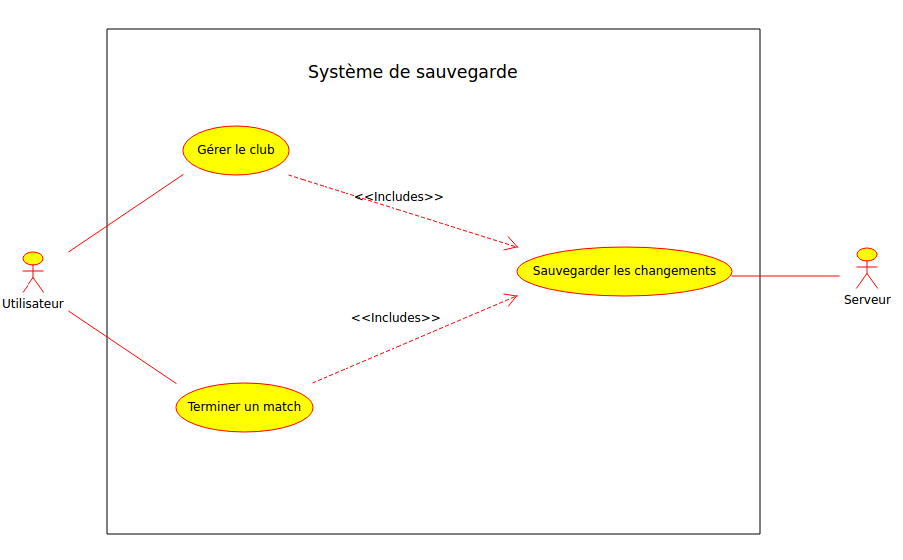
\includegraphics[height=250pt]{uml/svg.png}
   \end{center}
\end{figure}
\begin{description}
\item[Cas général :] Le système doit sauvegarder tout changement effectué au \gls{club} durant la phase management ainsi qu'après une partie.
\item[Pré Condition  :] Une modification du \gls{club} en phase management, ou une fin de match.
\item[Post Condition :] Les changements apportés au \glspl{club} et au \gls{serveur} seront sauvegardés.
\item[Cas Exceptionnel :] Aucune sauvegarde ne sera effectuée par le module de sauvegarde si le \gls{serveur} plante.
\end{description}


\subsection{Exigences non fonctionnelles}
\label{enf}
\begin{itemize}
\item Le \gls{client} et le \gls{serveur} doivent être écrits en \textbf{C++} et seront compilés à l'aide de \textbf{gcc 4.8}
\item Le \gls{client} et le \gls{serveur} doivent être portables et pouvoir fonctionner sur un système \textbf{UNIX} et une architecture x86
\item La machine exécutant le \gls{serveur} doit être capable de gérer une connexion ouverte constamment vers chaque \gls{client} ainsi que de stocker l'entièreté des données du jeu en mémoire disque ainsi qu'une grande majorité en mémoire vive.
\end{itemize}

\subsection{Design et fonctionnement}
\begin{figure}[h]
   \caption{\label{3} Diagramme de classe représentant toutes les structures de données}
   \begin{center}
   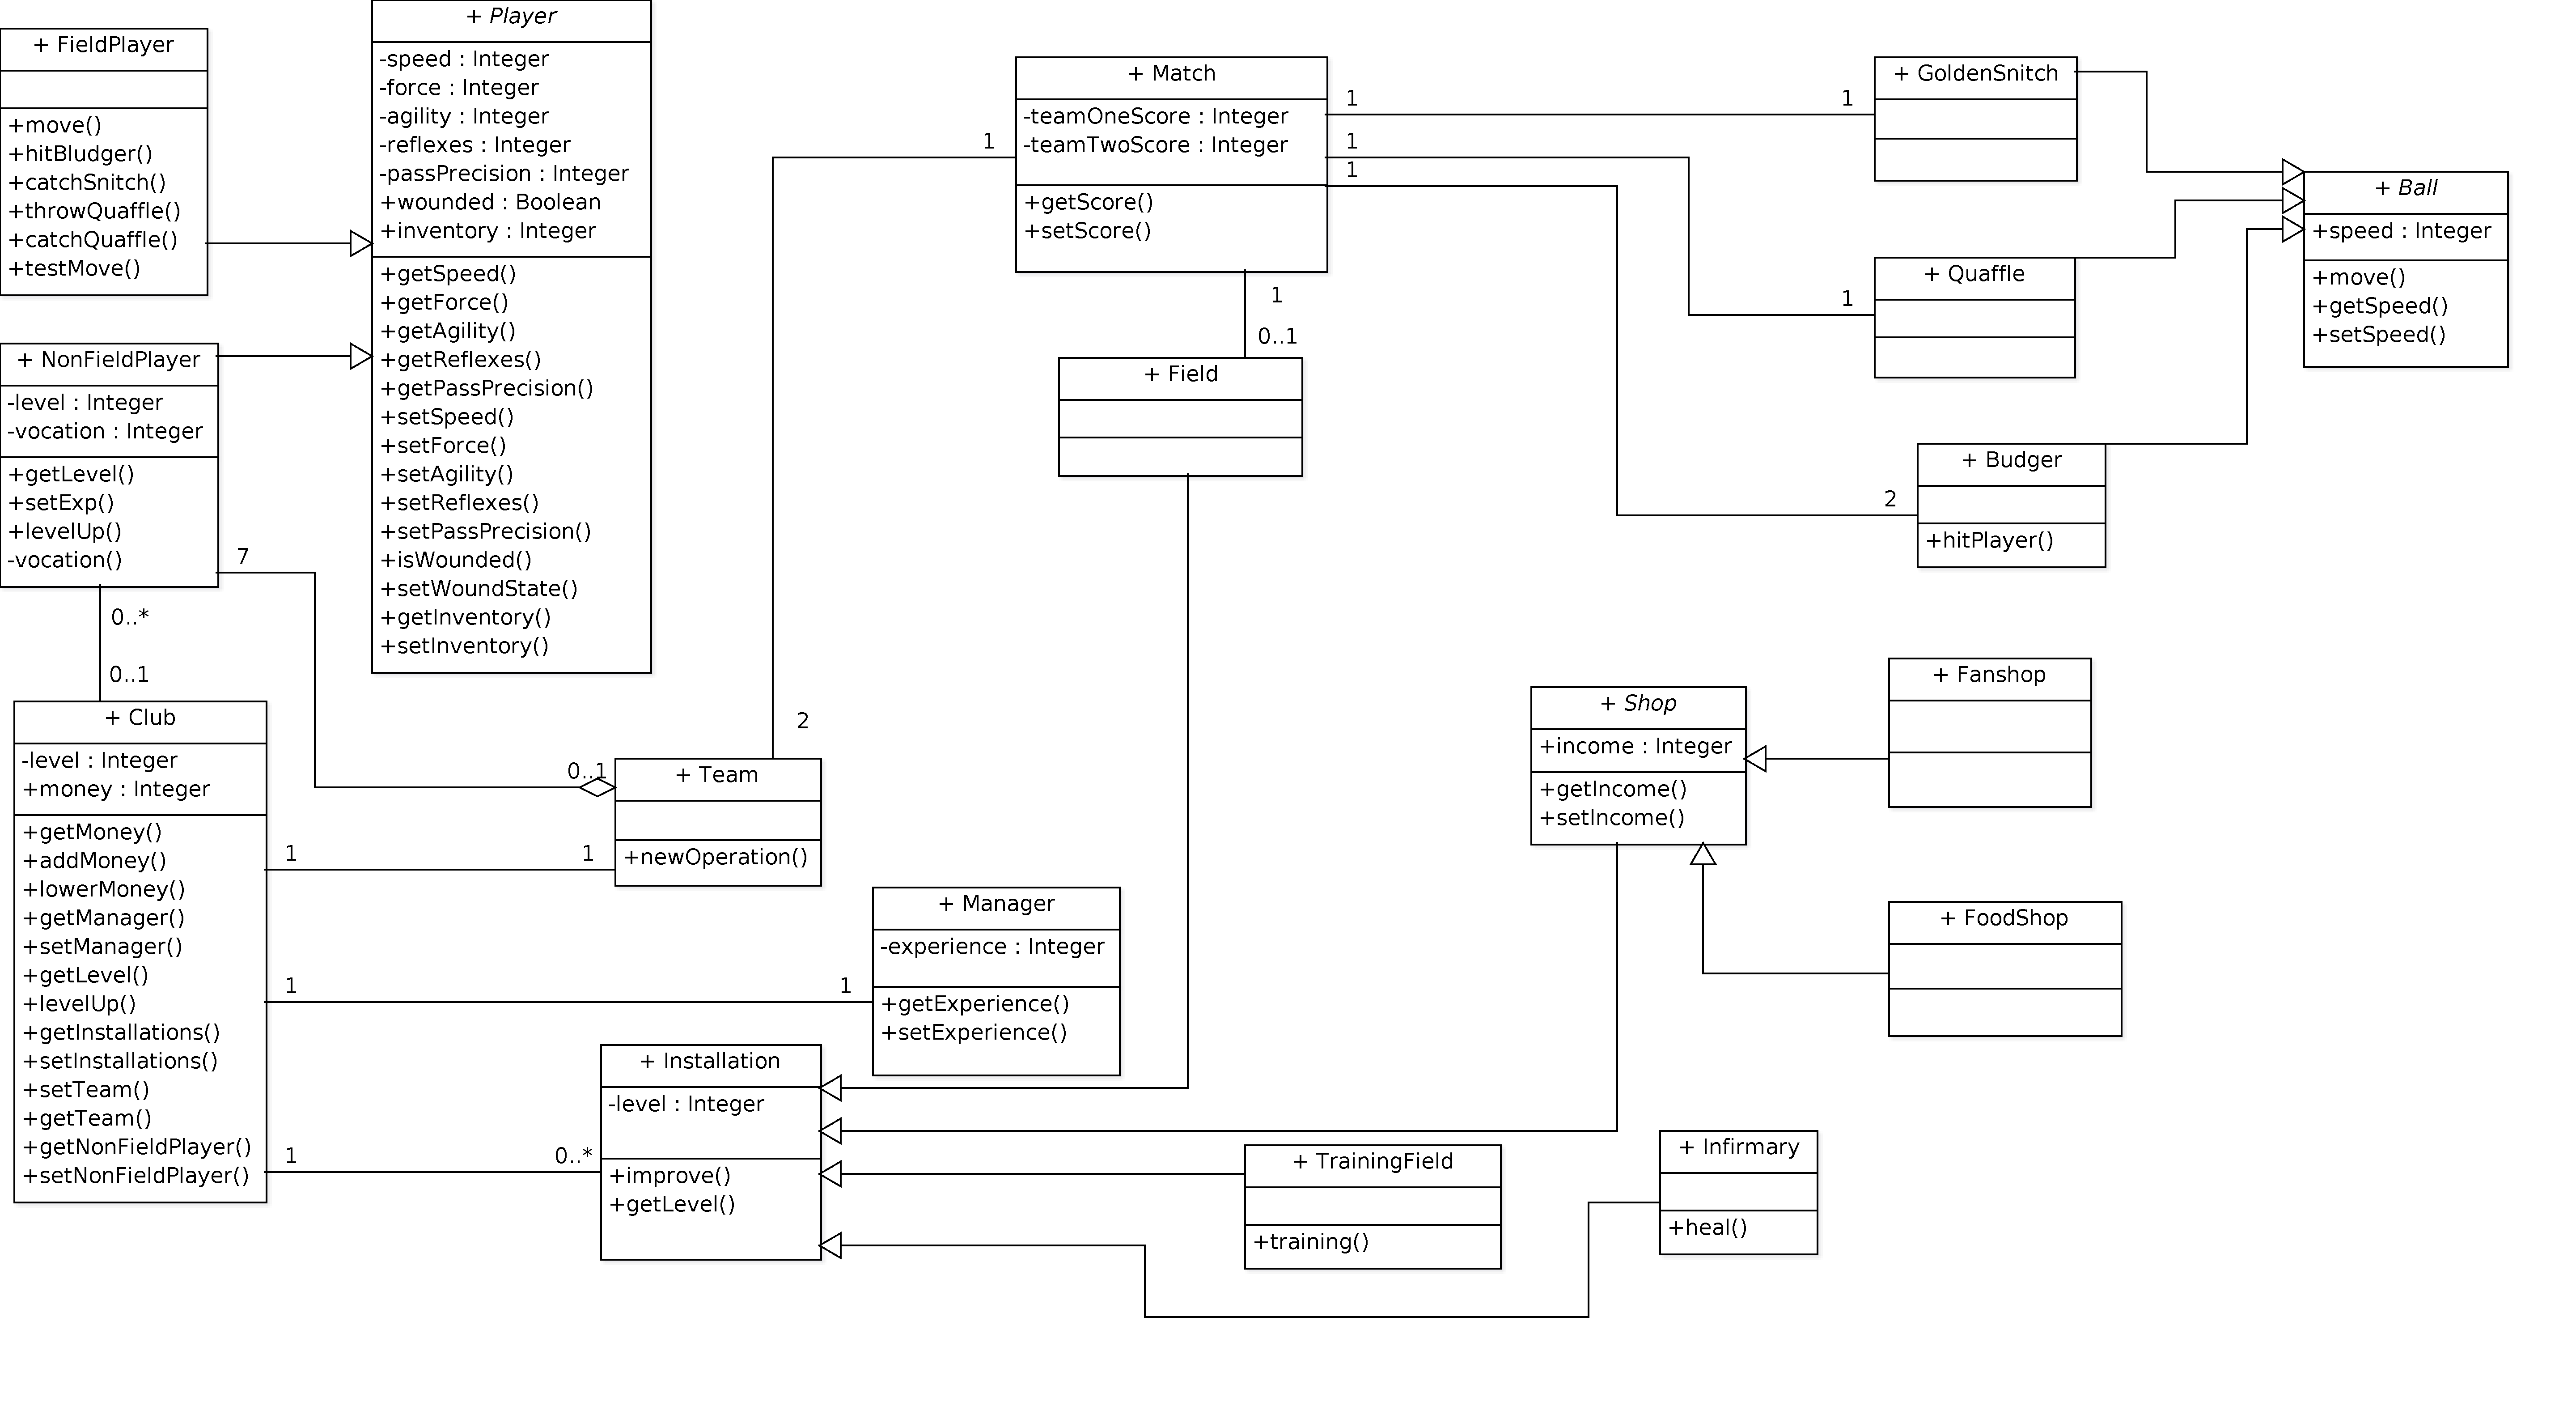
\includegraphics[height=250pt]{uml/classDiagram.png}
   \end{center}
\end{figure}

\printindex
\tableofcontents
\listoffigures
%\listoftables

\end{document}
